\chapter{Stereo Camera Depth Node Implementation}
\label{chapter:stereo_camera_depth}

First and foremost, to emphasize the advantages of range information given by a stereo camera the following comparison is performed:

\section{Implementation}

Like Structure from Motion, the stereo depth instance is a ROS node which is given images and image poses from the xVIO state estimator. As the state estimator was in its final development stages during my thesis, camera images and a ground truth camera pose from the simulation were used instead as input for the stereo algorithm. Note that only one camera pose is given as the second one is derived in a straight forward manner, given the fixed baseline.

The stereo depth implementation was done using OpenCV's StereoSGBM algorithm. As stereo depth generation is a widely known topic I won't go into the details here.

The final output of the node is a generated point cloud in the world frame together with two poses representing the camera locations of the generated point cloud.

\subsection{Transform Overview}

A critical part of navigation is always the consistency of the coordinate systems in which quantities are represented. Hereafter is a display of the present coordinate systems in the stereo camera setup.

\subsection{Landing Site Detection without Lateral Motion}

Taking off vertically with the drone in the simulation, the first landing site without lateral motion was found.

\begin{figure}
    \centering
    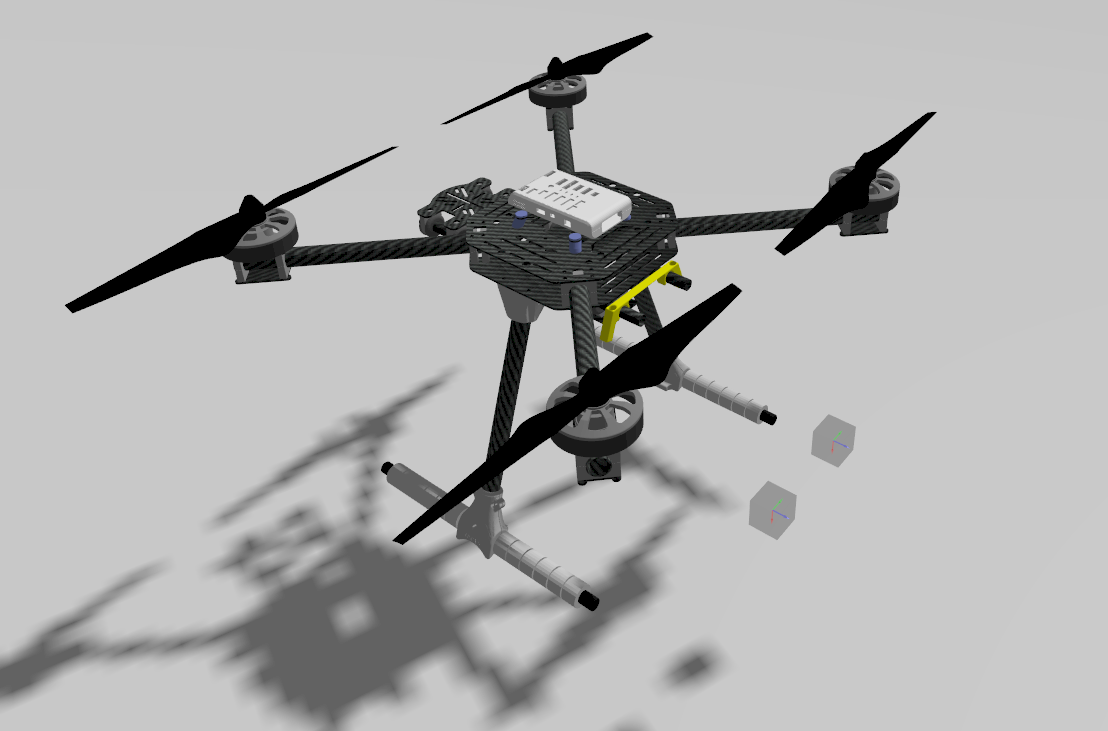
\includegraphics[scale=0.32]{images/preparation/stereo/drone_with_stereo_cam.png}
    \caption{Stereo camera on drone indicated by opaque boxes}
\end{figure}

\begin{figure}
    \centering
    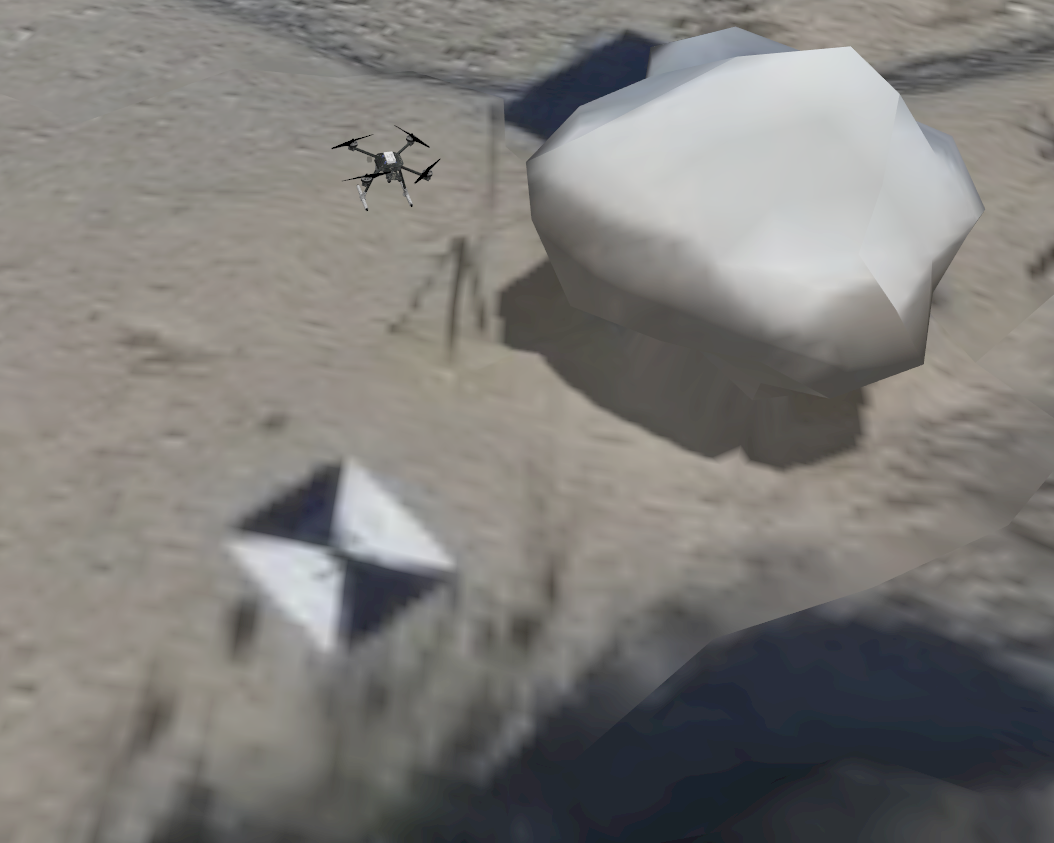
\includegraphics[scale=0.34]{images/preparation/stereo/ascent_sim.png}
    \caption{Drone during vertical ascent in simulation}
\end{figure}

\begin{figure}
    \centering
    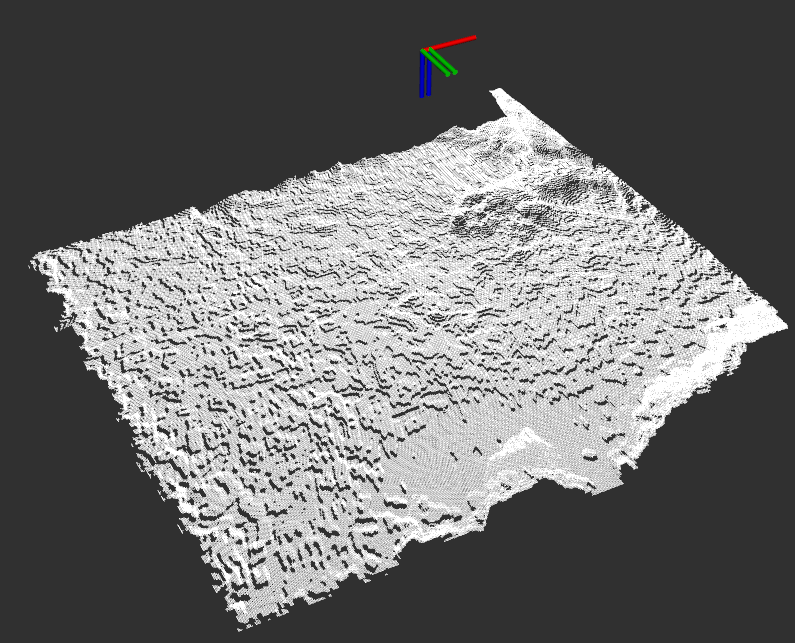
\includegraphics[scale=0.45]{images/preparation/stereo/stereo_pointcloud.png}
    \caption{RViz visualization of created point cloud from stereo camera}
\end{figure}
\clearpage %HERE

\begin{figure}
    \centering
    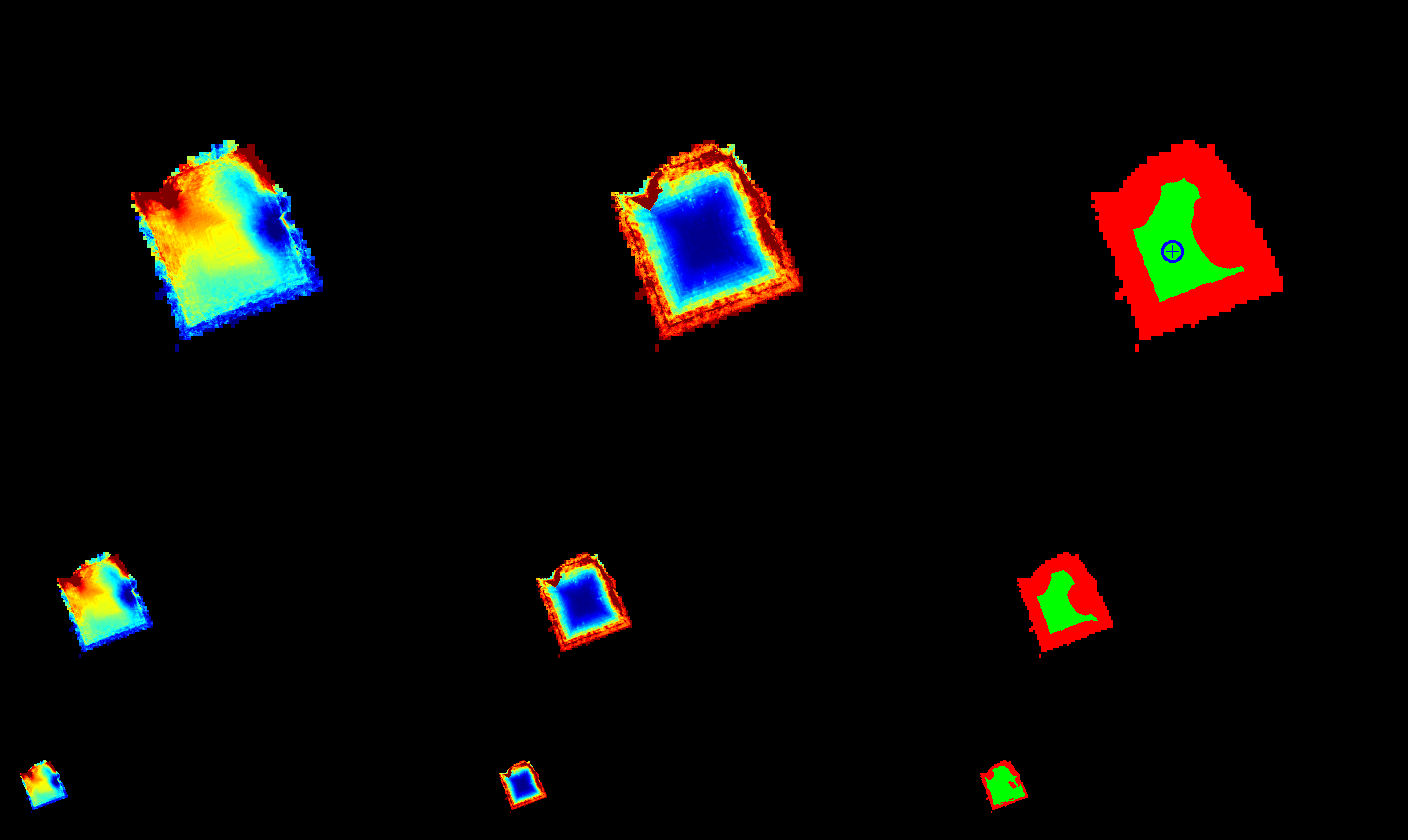
\includegraphics[scale=0.25]{images/preparation/stereo/lsd_ascent.png}
    \caption{LSD Debug output displaying LORNA's first detected landing site during vertical motion}
\end{figure}

\subsection{Switching}

In order to achieve the final desired perception mechanism of flying laterally with SFM and using a stereo camera depth node at low altitudes, one needs to switch between the two alternatives.

The obvious flag to use in the switching mechanism is the current altitude above ground. This could be achieved by analyzing the generated point cloud at a given iteration to determine the median altitude which indicates the altitude above ground. This however is avoidable computational overhead.

As mentioned in \cref{sec:state_estimator} the drone has a laser range finder on board. This allows us to get an estimate of the altitude above ground at any given moment without the need for image processing.

Therefore, the switching is performed by using a separate ROS subscriber which continuously checks the LRF's measurement and activates or deactivates the SFM node and stereo node respectively.

\clearpage %HERE
\begin{figure}
    \centering
    \includegraphics[scale=0.17]{images/preparation/stereo/switching.png}
    \caption{Laser Ranger Finder Based Switch between Depth Sources}
\end{figure}

\section{Qualitative Practical Analysis}

Once implemented the landing site detection instance could be supplied by the stereo depth node. The result thereof can be seen below:

\begin{figure}[ht!]
    \centering
    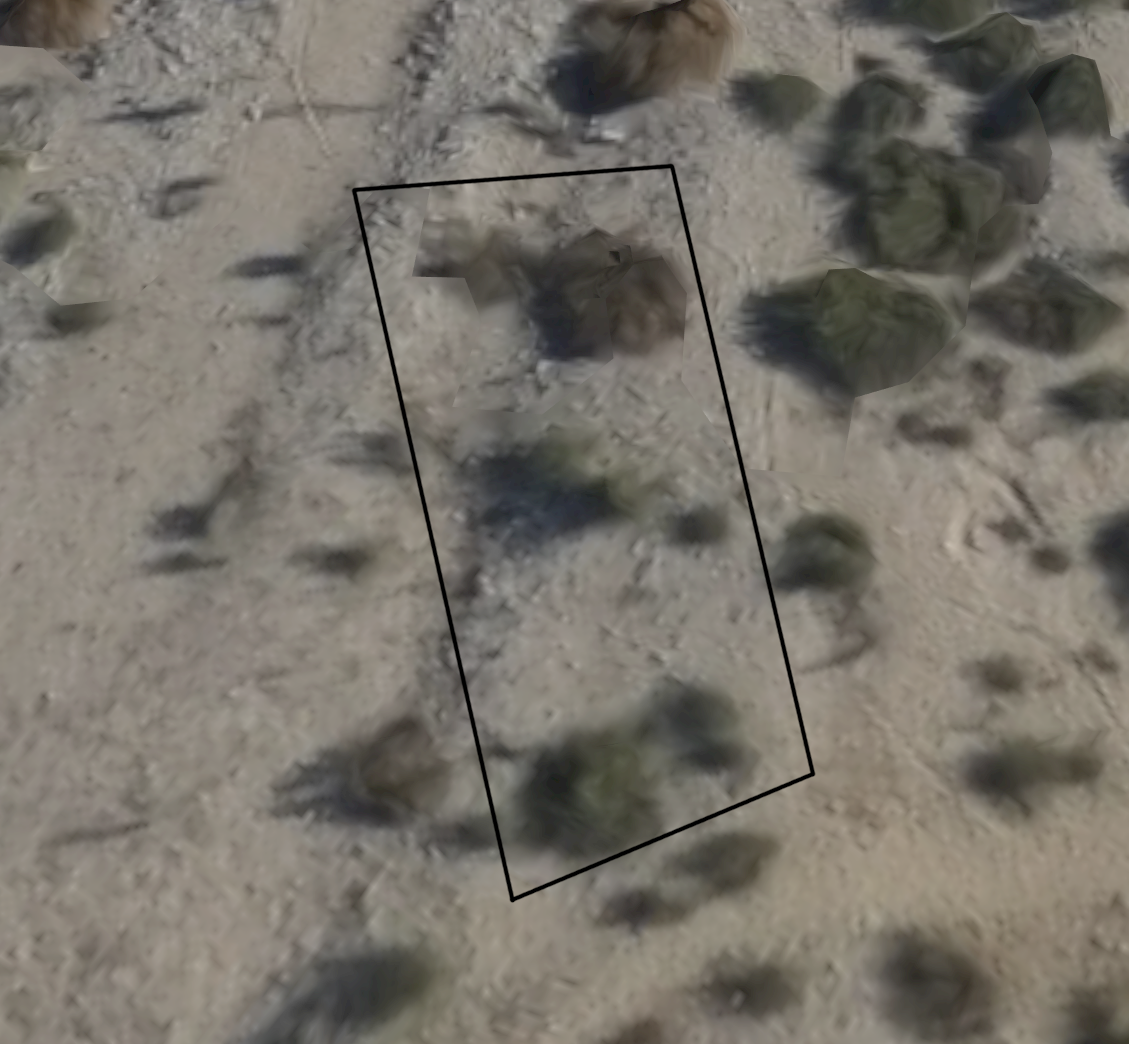
\includegraphics[scale=0.2, angle=-12]{images/preparation/reference_map2.5m_annotated.png}
    \caption{Considered terrain patch in Gazebo simulation}
    \label{stereo_reference}
\end{figure}

\begin{figure}[ht!]
    \centering
    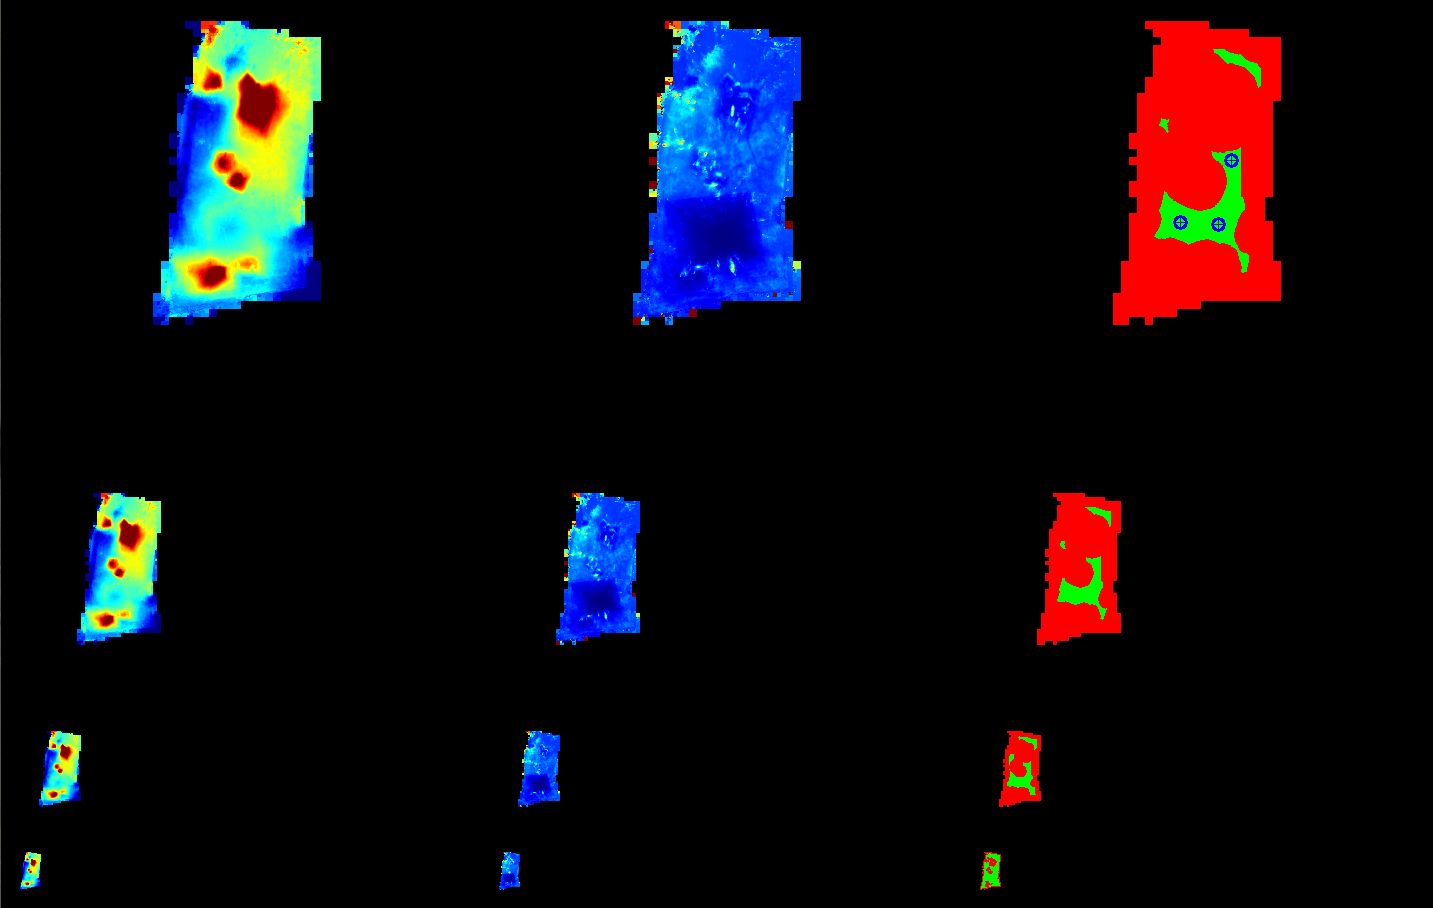
\includegraphics[scale=0.25]{images/preparation/stereo_2.5m.png}
    \caption{Stereo camera depth supplied LSD debug image at 2.5 m altitude}
    \label{qual_stereo_test}
\end{figure}

\clearpage %HERE

\begin{figure}[ht!]
    \centering
    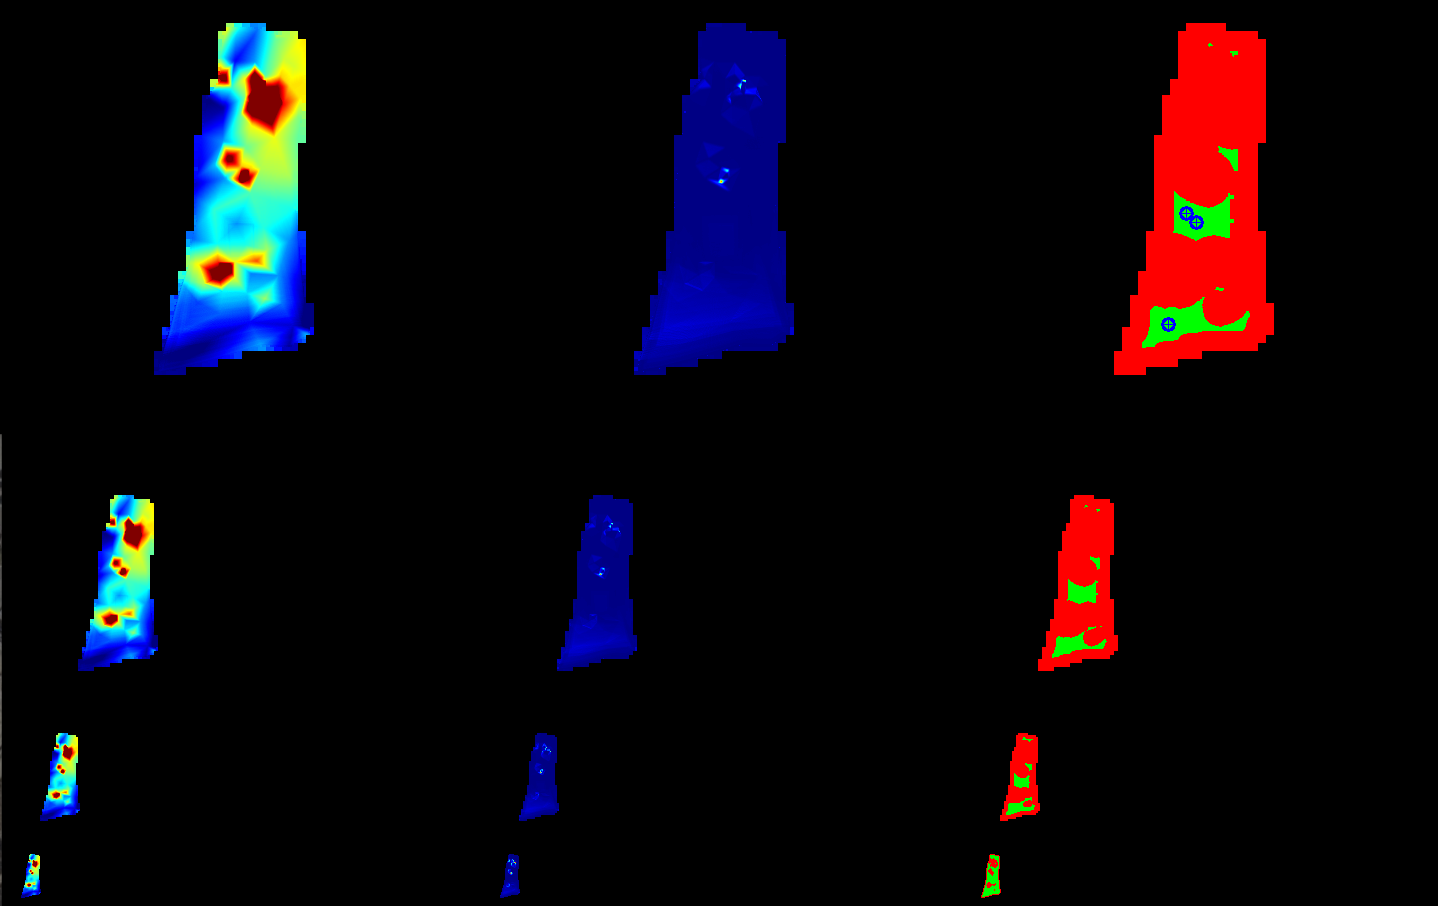
\includegraphics[scale=0.25]{images/preparation/GT_2.5m.png}
    \caption{GT depth supplied LSD debug image at 2.5 m altitude}
    \label{stereo_GT}
\end{figure}

When comparing the result to the ground truth LSD output it can be seen that LSD creates a very accurate DEM from the stereo camera depth input. The landing sites detected are reasonable when compared to the terrain reference. 




